%卒論概要テンプレート ver. 4.0

\documentclass[uplatex,twocolumn,dvipdfmx]{jsarticle}
\usepackage[top=22mm,bottom=22mm,left=22mm,right=22mm]{geometry}
\setlength{\columnsep}{11mm}
\usepackage[T1]{fontenc}
\usepackage{txfonts}
\usepackage[expert,deluxe]{otf}
\usepackage[dvipdfmx,hiresbb]{graphicx}
\usepackage[dvipdfmx]{hyperref}
\usepackage{pxjahyper}
\usepackage{secdot}





%タイトルと学生番号,名前だけ編集すること
\title{\vspace{-5mm}\fontsize{14pt}{0pt}\selectfont Twitterにおけるデマ拡散のシミュレーション}
\author{\normalsize プロジェクトマネジメントコース 矢吹研究室 1442043 川崎貴雅}
\date{}
\pagestyle{empty}
\begin{document}
\fontsize{10.5pt}{\baselineskip}\selectfont
\maketitle



%以下が本文
\section{序論}\label{序論}

Twitterはリアルタイムな情報を手軽に多くのユーザへと伝播できるため社会に影響を与えている.\#MeTooというハッシュタグの投稿により性的被害やセクハラについて考えるきっかけが,世界中に広がった事が挙げられる.
しかし悪い影響を与えてしまう場合もある.例えば東日本大震災時のデマ情報が拡散された事や北朝鮮のミサイルを目撃したというデマが挙げられる.このようなツイートの拡散をシミュレーションで再現することを試みる.
本研究ではTwitterのデマ拡散をシミュレーションで再現することができるかの調査を行う.

\section{目的}

本研究では現実のデマ拡散に近い状況を再現できるシミュレーションの開発である.

\section{手法}

デマの拡散をシミュレートするためには,ユーザ同士のネットワーク作成,つぶやきの頻度,RTの頻度を求めることが必要なため,以下の手順で行う.
\begin{enumerate}
\item ツイートの拡散する様子をシュミレートする手法を確立するために,ランダムグラフでのRTシミュレーションを試みる\cite{netto}.
\item TwitterAPIを用いて50万人のユーザから1日のツイート数取得を行い,それをもとに1日あたりのツイート数の分布を出す.
\item ユーザから一日のRT数の取得を行い,分布を出す
\item ユーザ間のフォロー関係のデータを取得しその平均を出す.
\end{enumerate}

\section{結果}

50万人のデータから1日あたりのツイート数の分布が分かった.またグループ構築にランダムグラフを使ったツイート拡散のシュミレート手法も確立できた.図\ref{何人がRTを見るか}のようにフォロー数とRTをするかの数値を動かして可視化を行えるようになった.しかし1日あたりのRT数の分布とユーザのフォロー関係が出せなかったため現実的なシミュレーションを行うことはできなかった.

\begin{figure}[htb]
\centering
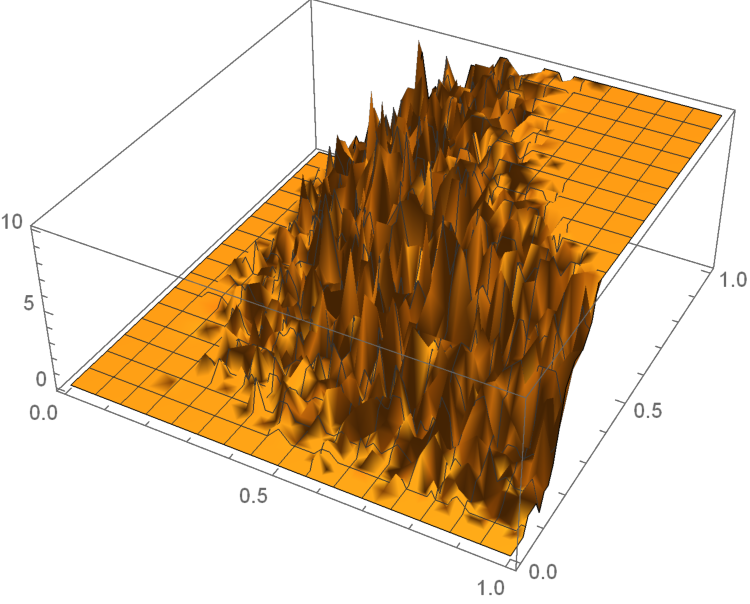
\includegraphics[width=44mm,clip]{result.pdf}
\caption{x軸が繋がっている確率,y軸がRTをする確率,z軸が人数のシミュレーションの結果}\label{何人がRTを見るか}
\end{figure}

\section{考察}

10人でのシミュレーションのメンバ全てがツイートを確認できるようになるのは互いに繋がってる確率が0.5でRTする確率が0.6であると分かった.またメンバが増えると全メンバ確認するまでにフォローとRTの確率それぞれが下がったため,メンバ数の増加は拡散力をあげると考えられる.

\section{結論}

本研究では,1日あたりのツイート数の分布とツイート拡散のシュミレートをする手法の確立を行った.その結果1日のあたりのツイート数の分布確認,ツイートの拡散シミュレートの手法の確立が行えた.この結果に1日あたりのRT数の分布とユーザ間のフォロー関係のデータが取得できれば現実に近いシミュレーションを行うことが期待できる.

\bibliographystyle{junsrt}
\bibliography{biblio}%「biblio.bib」というファイルが必要.

\end{document}
